% Template for a Computer Science Tripos Part II project dissertation
\documentclass[12pt,a4paper,twoside,openright]{report}
\usepackage[pdfborder={0 0 0}]{hyperref}    % turns references into hyperlinks
\usepackage{geometry}  % adjusts page layout
\usepackage{graphicx}  % allows inclusion of PDF, PNG and JPG images
\usepackage{verbatim}
\usepackage{docmute}   % only needed to allow inclusion of proposal.tex
\usepackage[style=numeric-comp, backend=bibtex]{biblatex}
\usepackage[UKenglish]{babel}
\usepackage[parfill]{parskip}
\usepackage{tabu}
\usepackage{siunitx}
\usepackage{amsfonts}
\usepackage{amsmath}

\addbibresource{refs.bib}

% \raggedbottom                           % try to avoid widows and orphans
% \sloppy
% \clubpenalty1000%
% \widowpenalty1000%
\graphicspath{ {figs/} }
% \renewcommand{\baselinestretch}{1.1}    % adjust line spacing to make
                                        % more readable
\renewcommand*\rmdefault{ppl}

% New definition of square root:
% it renames \sqrt as \oldsqrt
% \let\oldsqrt\sqrt
% % it defines the new \sqrt in terms of the old one
% \def\sqrt{\mathpalette\DHLhksqrt}
% \def\DHLhksqrt#1#2{%
% \setbox0=\hbox{$#1\oldsqrt{#2\,}$}\dimen0=\ht0
% \advance\dimen0-0.2\ht0
% \setbox2=\hbox{\vrule height\ht0 depth -\dimen0}%
% {\box0\lower0.4pt\box2}}
        
\begin{document}



%%%%%%%%%%%%%%%%%%%%%%%%%%%%%%%%%%%%%%%%%%%%%%%%%%%%%%%%%%%%%%%%%%%%%%%%
% Title


% \pagestyle{empty}
%
% \rightline{\LARGE \textbf{Martin Richards}}
%
% \vspace*{60mm}
% \begin{center}
% \Huge
% \textbf{How to write a dissertation in \LaTeX} \\[5mm]
% Computer Science Tripos -- Part II \\[5mm]
% St John's College \\[5mm]
% \today  % today's date
% \end{center}

%%%%%%%%%%%%%%%%%%%%%%%%%%%%%%%%%%%%%%%%%%%%%%%%%%%%%%%%%%%%%%%%%%%%%%%%%%%%%%
% Proforma, table of contents and list of figures

% \pagestyle{plain}
%
% \chapter*{Proforma}
%
% {\large
% \begin{tabular}{ll}
% Name:               & \bf Martin Richards                       \\
% College:            & \bf St John's College                     \\
% Project Title:      & \bf How to write a dissertation in \LaTeX \\
% Examination:        & \bf Computer Science Tripos -- Part II, July 2001  \\
% Word Count:         & \bf 1587\footnotemark[1]
%                       (well less than the 12000 limit)  \\
% Project Originator: & Dr M.~Richards                    \\
% Supervisor:         & Dr Markus Kuhn                    \\
% \end{tabular}
% }
% \footnotetext[1]{This word count was computed
% by \texttt{detex diss.tex | tr -cd '0-9A-Za-z $\tt\backslash$n' | wc -w}
% }
% \stepcounter{footnote}
%
%
% \section*{Original Aims of the Project}
%
% To write a demonstration dissertation\footnote{A normal footnote without the
% complication of being in a table.} using \LaTeX\ to save
% student's time when writing their own dissertations. The dissertation
% should illustrate how to use the more common \LaTeX\ constructs. It
% should include pictures and diagrams to show how these can be
% incorporated into the dissertation.  It should contain the entire
% \LaTeX\ source of the dissertation and the makefile.  It should
% explain how to construct an MSDOS disk of the dissertation in
% Postscript format that can be used by the book shop for printing, and,
% finally, it should have the prescribed layout and format of a diploma
% dissertation.
%
%
% \section*{Work Completed}
%
% All that has been completed appears in this dissertation.
%
% \section*{Special Difficulties}
%
% Learning how to incorporate encapulated postscript into a \LaTeX\
% document on both Ubuntu Linux and OS X.
%
% \newpage
% \section*{Declaration}
%
% I, George Thomas of Peterhouse, being a candidate for Part II of the Computer
% Science Tripos, hereby declare
% that this dissertation and the work described in it are my own work,
% unaided except as may be specified below, and that the dissertation
% does not contain material that has already been used to any substantial
% extent for a comparable purpose.
%
% \bigskip
% \leftline{Signed [signature]}
%
% \medskip
% \leftline{Date [date]}
%
% \tableofcontents
%
% \listoffigures
%
% \newpage
% \section*{Acknowledgements}
%
% This document owes much to an earlier version written by Simon Moore.  His help, encouragement and advice was greatly
% appreciated.

%%%%%%%%%%%%%%%%%%%%%%%%%%%%%%%%%%%%%%%%%%%%%%%%%%%%%%%%%%%%%%%%%%%%%%%
% now for the chapters

\pagestyle{headings}

\chapter{Introduction}
  This dissertation describes the implementation and evaluation of an activity classifier using 
  accelerometer data captured simutaneously from a smartphone and a smartwatch.  
  
  The classifier using data from both sources outperforms a classifier using only smartphone data,
  and the classifier that uses only smartphone data outperforms a classifier using only smartwatch 
  data.
  \section{Motivation}
  \label{sec:intro-motivation}
    Wearable devices are set to become the next big technology trend. Wrist-worn wearables, 
    including smartwatches, formed the majority of the 21m wearable devices sold year. Analysts
    predict the Apple Watch will sell between 20m and 40m in its first nine months 
    \cite{econapplewatch}.
    
    One of the primary appeals of wearables is their ability to sense. Like smartphones before them,
    smartwatches will enhance the ability to collect data about people. This data is important to
    consumers, who purchase specialised wearables to measure activity, sleep patterns and 
    caloric intake. The data's research potential is also laudable --- Apple's ResearchKit will
    allow medical researchers to access data about their patients with greater ease than ever
    before \cite{appleresearchkit}.
        
    Accurate activity classification therefore has many academic and commercial applications. To be
    marketable, activity classification solutions must use current consumer devices. Though 
    rudimentary activity classification is available on Android smartphones, an approach that
    utilises simutaneous collection from a smartphone and smartwatch has not been investigated in
    any detail.
     
    This dissertation details the implemenation of accelerometer data collection using current 
    consumer devices (an Android smartphone and Android Wear smartwatch), classifies a user's 
    activities and compares this classification accuracy to using only smartphone data and using 
    only smartwatch data. 
    
  \section{Challenges}
  \label{sec:intro-challenges}
    This project requires knowledge of a variety of disparate areas in computer science. 
    
    Writing software for mobile devices requires knowledge of their paradigms and nuances.
    Mobile devices are also subject to battery life and computational power constraints and   
    particular care must be taken to build a solution that works in practice.  
    A project that utilises built-in sensors also requires an understanding of the features and 
    limitations of those sensors and good knowledge in the APIs that are provided to access them.

    The sensors also output data at a high rate and care must be taken to correctly handle the
    performance and concurrency issues that may arise. Storage and transfer of large amounts of
    raw data, especially on a memory-limited device such as a smartwatch, also requires special
    consideration. 
    
    The data processing aspects of the project will require an understanding of digital signal 
    processing, Fourier methods, artificial intelligence and machine learning, and statistics.
  
  \section{Related Work}
  \label{sec:intro-relatedwork}
    Activity classification using accelerometer data from body-mounted devices is not a new topic: 
    Bao et al. \cite{bao2004activity} detect physicial activities using five biaxial acceleometers
    worn on different parts of the body. 
    
    Long et al. \cite{long2009single} use a single tri-axial accelerometer placed on the wrist and 
    use it to achieve an $80\%$ activity classification accuracy in five activities. One of the
    more interesting highlights of Long et al. is that only $50\%$ of all cycling in correctly
    classified.
    
    


\chapter{Preparation}
  This chapter details the work done before the main implementation of the project was started. It
  details the devices chosen to implement this project and the reasons for choosing them. It then
  discusses the existing libraries and APIs available for those devices and for the required data
  processing. The design decisions are supported by some preliminary results on sensor noise.  Finally, it describes software engineering techniques used.

  \section{Requirements analysis}
    The aim of the project is to classify activities based on accelerometer recordings from a consumer smartwatch and smartphone, and evaluate to what extent the smartwatch is better at helping to classify activities. The requirements to accomplish this can be split into two categories: data collection and data processing requirements.
    
    \subsubsection{Data collection requirements}
      \begin{enumerate}
        \item access tri-axial readings from accelerometer on both the smartwatch and the smartphone;
        \item store this accelerometer data temporarily on the internal memory of each device using suitable data structures;
        \item transmit this data from the smartwatch to the smartphone using a suitable protocol, because of memory constraints and to enable transfer to a;
        \item store the data permanently on the smartphone.
      \end{enumerate}
    
    \subsubsection{Data processing requirements}
      \begin{enumerate}
        \item parse the data into a manipulatable format;
        \item preprocess the data, including filtering and splitting into fixed-length bins;
        \item extract features from each bin;
        \item train classifier(s) on the extracted features;
        \item test classifier and record evaluation statistics.
      \end{enumerate}
    
    The remainder of this chapter describes work done to ensure these requirements could be fulfilled.
  
  \section{Hardware devices}
    The success of this project depends partly on correct selection and understanding of the devices
    used to collect data. Both the smartwatch and the smartphone are required to contain accelerometers accessible to
    developers.
    
    Android devices were chosen as Android Wear was the most mature platform for developing with
    wearable devices at the time. It runs on the widest variety of devices and provides developer 
    access to its sensors.
    
    \subsection{Smartphone}
      The smartphone chosen for development was the Google Nexus 5. Smartphone technology has
      advanced to the point that many Android smartphones are homogeneous with respect to this
      project --- they all contain sufficient processing power, internal memory and an 
      accelerometer capable of recording data.
      
      The Nexus 5 contains a tri-axial accelerometer capable of recording measurements $\pm2\si{g}$
      on each axis, where $\si{g} \approx 9.81\si{\metre\per\square\second}$. This gives a total possible magnitude of $\sqrt{3 \times (2\mathrm{g})^2} = 2\mathrm{g}\sqrt{3} \approx 34 \si{\metre\per\square\second}$. Many other smartphones are susceptible to this limit and it is not thought that this will be an issue for classification.
      
      Figure~\ref{fig:nexus-5-accelerometer} shows the front face of a Nexus 5 with the axes of the
      accelerometer labeled.
      
      \begin{figure}[!th]
        \centering
        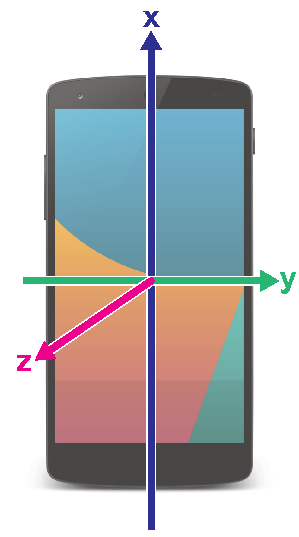
\includegraphics[width=0.3\textwidth]{Nexus_5_Accelerometer}
        \caption[A Nexus 5 device, overlaid with the coordinate system used by the Android API.]{A Nexus 5 device, overlaid with the coordinate system used by the Android API. The positive $x$ direction is defined as towards the top of the phone, the positive $y$ direction is defined as towards the right of the phone and the positive $z$ direction comes out of the screen. These directions are all relative to the natural portrait orientation of the device; they do not change when the device is used in horizontal orientation.}
        \label{fig:nexus-5-accelerometer}
      \end{figure}
      
      %TODO: include tech specs of Nexus 5?
    
    \subsection{Smartwatch}
      \label{sec:smartwatch}
      The smartwatch chosen for development was the Samsung Galaxy Gear Live, running Android Wear.
      It pairs to any device running Android 4.4 or higher and communicates over Bluetooth.
      
      Wearable devices that do not run Android typically run either Tizen, an open-source but not 
      widely adopted operating system, such as the Samsung Galaxy Gear 2, or a proprietary 
      operating system that does not allow access to the raw accelerometer data, for example the 
      Jawbone Up, and therefore cannot be used to compare classification accuracy with smartphones.
      
      There is more differentiation in smartwatches than there is in smartphones, with them varying
      not just in screen size but also in screen format (round or rectangular), battery life,
      charging facilities and sensors. Table~\ref{tab:smartwatch-features} presents an overview of possible smartwatch devices.
      
      Though the Sony Smartwatch 3 has the best technical stats, it wasn't yet fully released at the time we acquired the smartwatch. The group has had previous success with Samsung devices and the Gear Live met all the requires I had of the smartwatch for the project.
      \begin{table}
        \centering
        {\tabulinesep=1.2mm
        \begin{tabu} to \linewidth { p{2cm} X[l] X[l] X[l] X[l]}
          Device & \textbf{Samsung Galaxy Gear Live} & \textbf{Samsung Galaxy Gear 2} &\textbf{ LG G Watch} & \textbf{Sony Smartwatch 3} \\
          \hline
          Operating System & Android Wear & Tizen & Android Wear & Android Wear \\
          \hline
          Processor & 1.2 GHz single-core Qualcomm Snapdragon 400 & 1.0 GHz dual-core Exynos 3250 & 1.2 GHz single-core Qualcomm Snapdragon 400 & 1.2 GHz quad-core ARM A7 \\
          \hline
          Memory & 512 MB RAM & 512 MB RAM & 512 MB RAM & 512 MB RAM \\
          \hline
          Storage & 4 GB & 4 GB & 4 GB & 4 GB \\
          \hline
          Sensors & Touchscreen, Accelerometer, Gyroscope, Compass, Heart Rate Monitor & Touchscreen, Accelerometer, Gyroscope, Heart Rate Sensor, 2 MP Camera & Touchscreen, Accelerometer, Gyroscope, Compass & Touchscreen, Accelerometer, Gyroscope, Compass \\
          \hline
          Radios & Bluetooth 4.0 Low Energy & Bluetooth 4.0 Low Energy & Bluetooth 4.0 Low Energy & Bluetooth 4.0 Low Energy, GPS, NFC, Wi-Fi \\
          \hline
          Battery & 300 mAh & 300 mAh & 400 mAh & 420 mAh \\
          \hline
          Notes &  & Pairs only with Samsung devices &  & \\
          \hline
          
        \end{tabu}}
        \caption[An overview of possible smartwatch devices]{An overview of possible smartwatch devices. The Samsung Galaxy Gear Live was the device eventually chosen.}
        \label{tab:smartwatch-features}
      \end{table}
  
  \section{Working with accelerometer signals}
    \label{sec:intro-sig-processing}
    The output from any accelerometer is a time-series representing its acceleration. Effectively extracting information from this time-series is central to the success of this project. Knowledge of signal processing is therefore critical.
    
    It is essential to capture as much of the movement as possible. Conversion from continuous 
    physical acceleration to a discrete time-series requires sampling. The Nyquist-Shannon sampling theorem states that a signal can be exactly reconstructed from its samples if the sample rate is greater than twice the highest frequency of the signal.
    
    The highest frequency of a physical activity is not well defined. The activities I hope to classify will vary in their periodicity. Some, like walking, will be very periodic, while others, like climbing, will have no period at all. Considering common period activities like cycling and walking, I anticipate that the frequencies that best describe movement will be present in the 0--5\si{Hz} range, and so will require sampling at a frequency of at least 10\si{Hz}.
    
    \subsubsection{Frequency domain analysis}
      Much of the analysis of the accelerometer readings will be done in the frequency domain. A time domain signal can be converted into the frequency domain using a Fourier transform.
      
      The discrete Fourier transform of a sequence of N complex numbers $f_0, f_1, \ldots, f_{N-1}$ is the sequence $F_k$, defined by:
      
      $$F_k = \sum\limits_{n=0}^{N-1} f_n \cdot \mathrm{e}^{-2\pi \mathrm{i} kn/N}$$
      
      The power spectral density, $PSD_k$, of a signal describes how power is distributed over different frequencies. One method of estimating the power spectral density is to take the square of the absolute value of the Fourier transform component:
      
      $$PSD_k = \|F_k\|^2$$
      
    \subsubsection{Noise and filtering}
      The readings from the accelerometer are subject to noise, exhibited in 
      Figure~\ref{fig:x_y_z_flat_plot}, which plots readings from the X, Y, and Z axes during an hour long recording with the chosen smartphone laying flat on a table.
      
      \begin{figure}
        \centering
        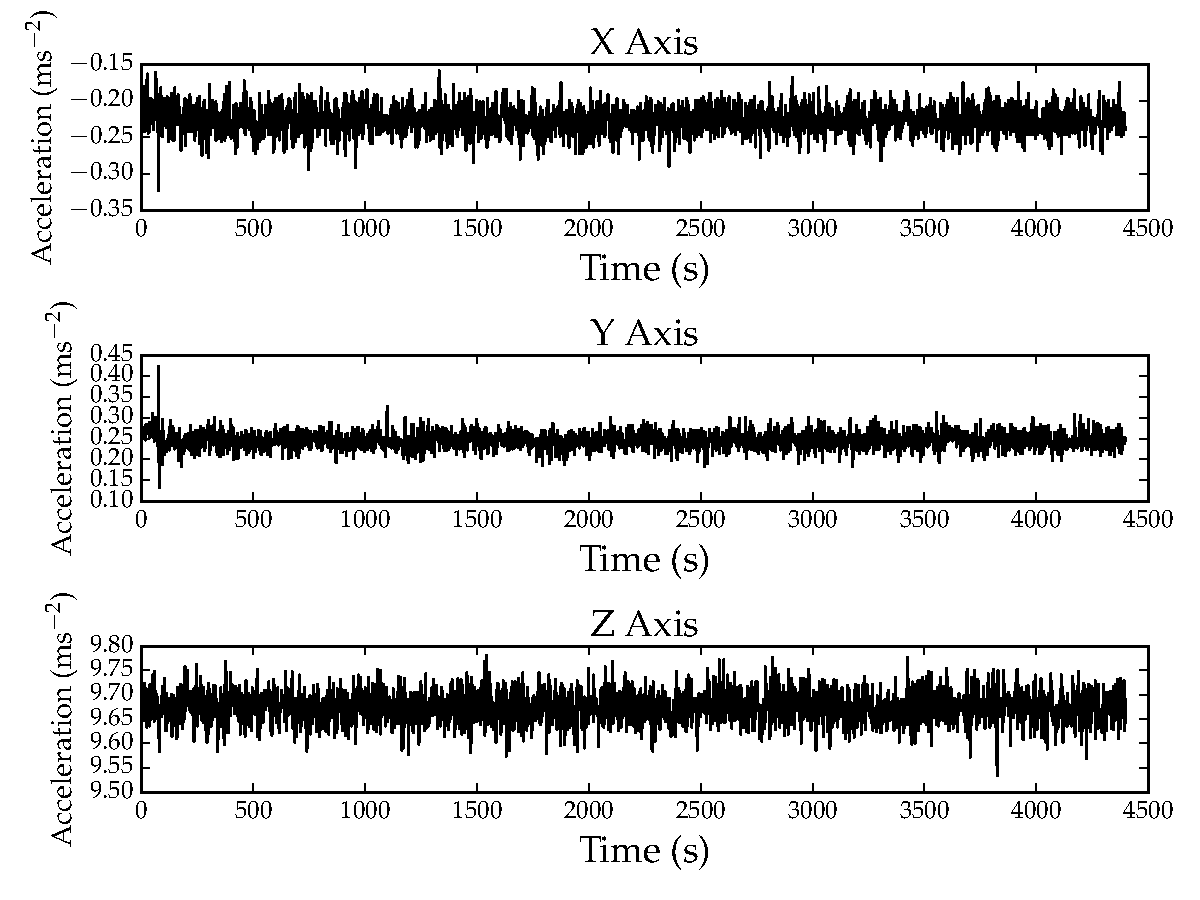
\includegraphics[width=1.0\textwidth]{x_y_z_flat_plot}
        \caption[Noisy readings of the X, Y and Z axes]{The X, Y and Z axis readings from an hour long accelerometer recording of the chosen smartphone laying flat on a table. The readings contain noise.}
        \label{fig:x_y_z_flat_plot}
      \end{figure}
      
      
      Figure~\ref{fig:noise_histogram} plots the distribution of the magnitude of the acceleration, where the magnitude $\|\mathbf{x}\| = \sqrt{x^2+y^2+z^2}$. The magnitude, which should be a constant $\mathrm{g} \approx 9.81 \si{\meter\per\square\second}$, is subject to normally distributed noise.
      
      \begin{figure}
        \centering
        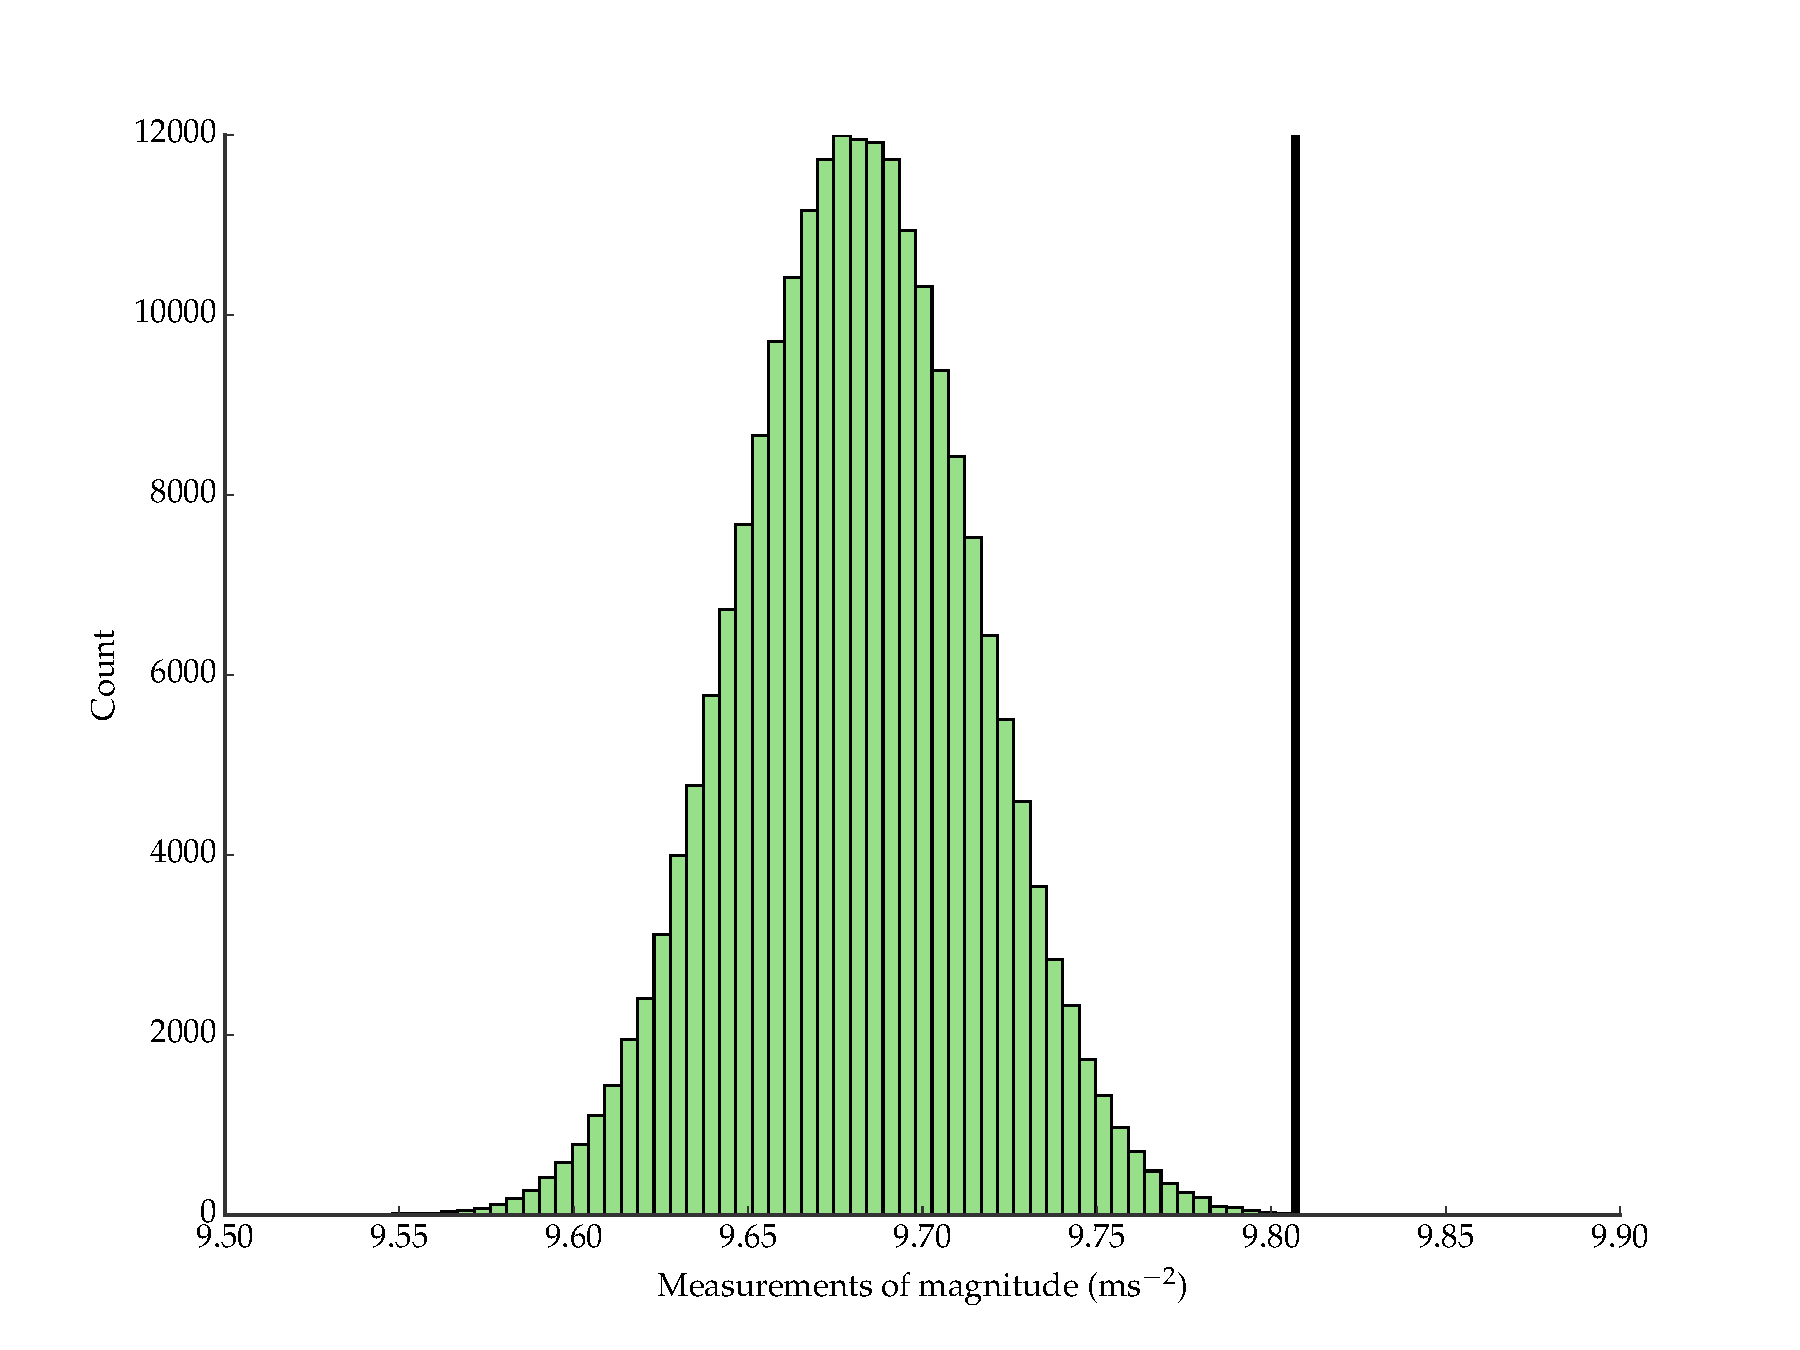
\includegraphics[width=1.0\textwidth]{noise_histogram}
        \caption[Histogram of the magnitude from the data shown in Figure~\ref{fig:x_y_z_flat_plot}.]{Histogram of the magnitude $\|\mathbf{x}\| = \sqrt{x^2+y^2+z^2}$ from the data shown in Figure~\ref{fig:x_y_z_flat_plot}. The magnitude should measure $ \mathrm{g} \approx 9.81\si{\metre\per\square\second}$, which is marked as the black dashed line on the graph. The noise implies the accelerometer data is imprecise. The mean of the data is less than $\mathrm{g}$, which indicates the recording is also inaccurate.}
        \label{fig:noise_histogram}
      \end{figure}
      
      Figure~\ref{fig:noise_prob_plot} gives a normal probability plot of the same magnitude data. Points on a normal probability plot should form a straight line if they are normally distributed. The straight line of best fit exhibits a coefficient of determination, $R^2 = 0.9993$, which is very close to 1. It is very likely that the noise is normally distributed.
      
      \begin{figure}
        \centering
        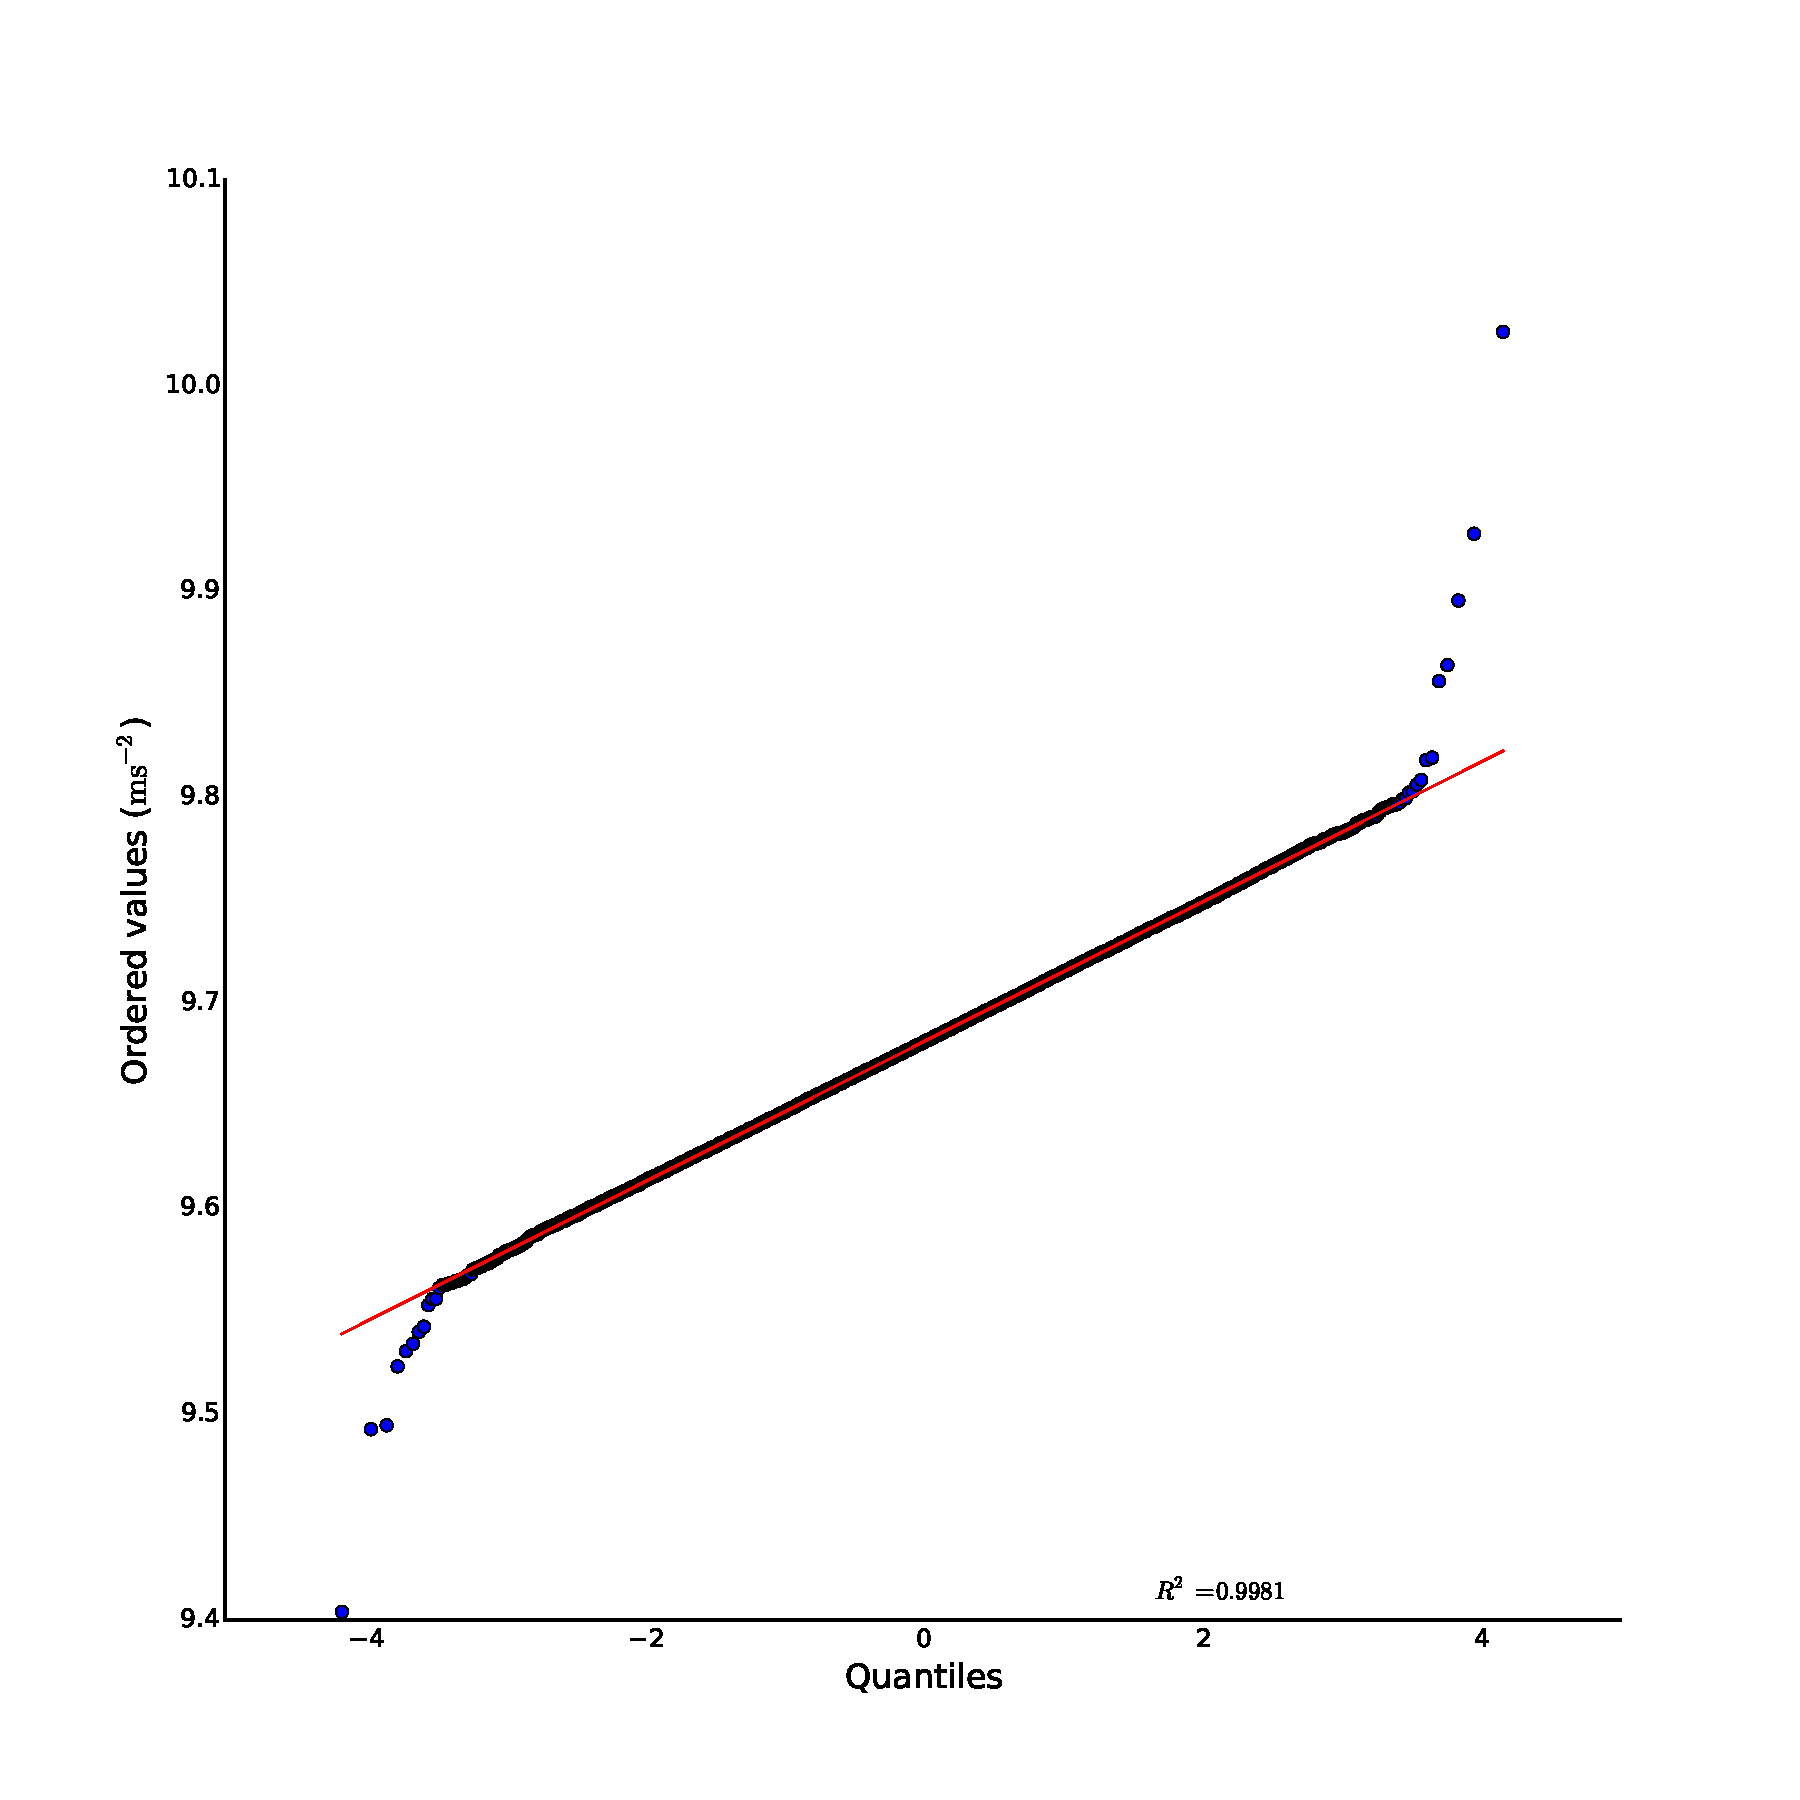
\includegraphics[width=1.0\textwidth]{noise_prob_plot}
        \caption[A normal probability plot of the magnitude from the data shown in Figure~\ref{fig:x_y_z_flat_plot}.]{A normal probability plot of the magnitude $\|\mathbf{x}\| = \sqrt{x^2+y^2+z^2}$  from the data shown in Figure~\ref{fig:x_y_z_flat_plot}. Data that is normally distributed will form a straight line when plotted in this way. This data is very likely to be normally distributed, as indicated by the straight line. ThThe straight line of best fit exhibits a coefficient of determination, $R^2 = 0.9993$}
        \label{fig:noise_prob_plot}
      \end{figure}
      
      %TOOD: http://docs.scipy.org/doc/scipy/reference/generated/scipy.stats.probplot.html
      
      Noise can be reduced with the application of a low-pass filter. A low-pass filter attenuates signals with a higher frequency than some cutoff, such as the noise exhibited in the signal. More information on low-pass filters in Section~\ref{sec:importing-and-preprocessing}.
      
      %TODO: explain how filters work?
  
  \section{Libraries and APIs}
      This project makes use of existing libraries and APIs for the data collection, data handling
      and classification aspects of the project. I investigate each library and API early on to ensure I don't encounter any potential show-stopping issues further along. 
    
    \subsection{Android Sensor API}
      \label{sec:sensor-api}
      The Android platform Sensor API\cite{androidsensoreventapi} is implemented using a publisher-subscriber model. Listeners must be registered
      to a particular sensor and must implement an \texttt{onSensorChanged()}
      method. The \texttt{onSensorChanged()} method is called whenever the sensor reports a new 
      value. A \texttt{SensorEvent} object is provided, containing a timestamp at which the data was
      reported together with the new data.
      
      The rate at which \texttt{onSensorChanged()} is called is `user-suggested'; though it can be 
      specified by the user, it can also be altered by the Android system. In practice, this means
      that the difference in timestamps is not constant but is approximately equal to the specified 
      delay. A histogram of timestamp differences for a particular 1 hour recording is given in 
      figure~\ref{fig:timestamp-differences}.
      
      \begin{figure}[h]
        \centering
        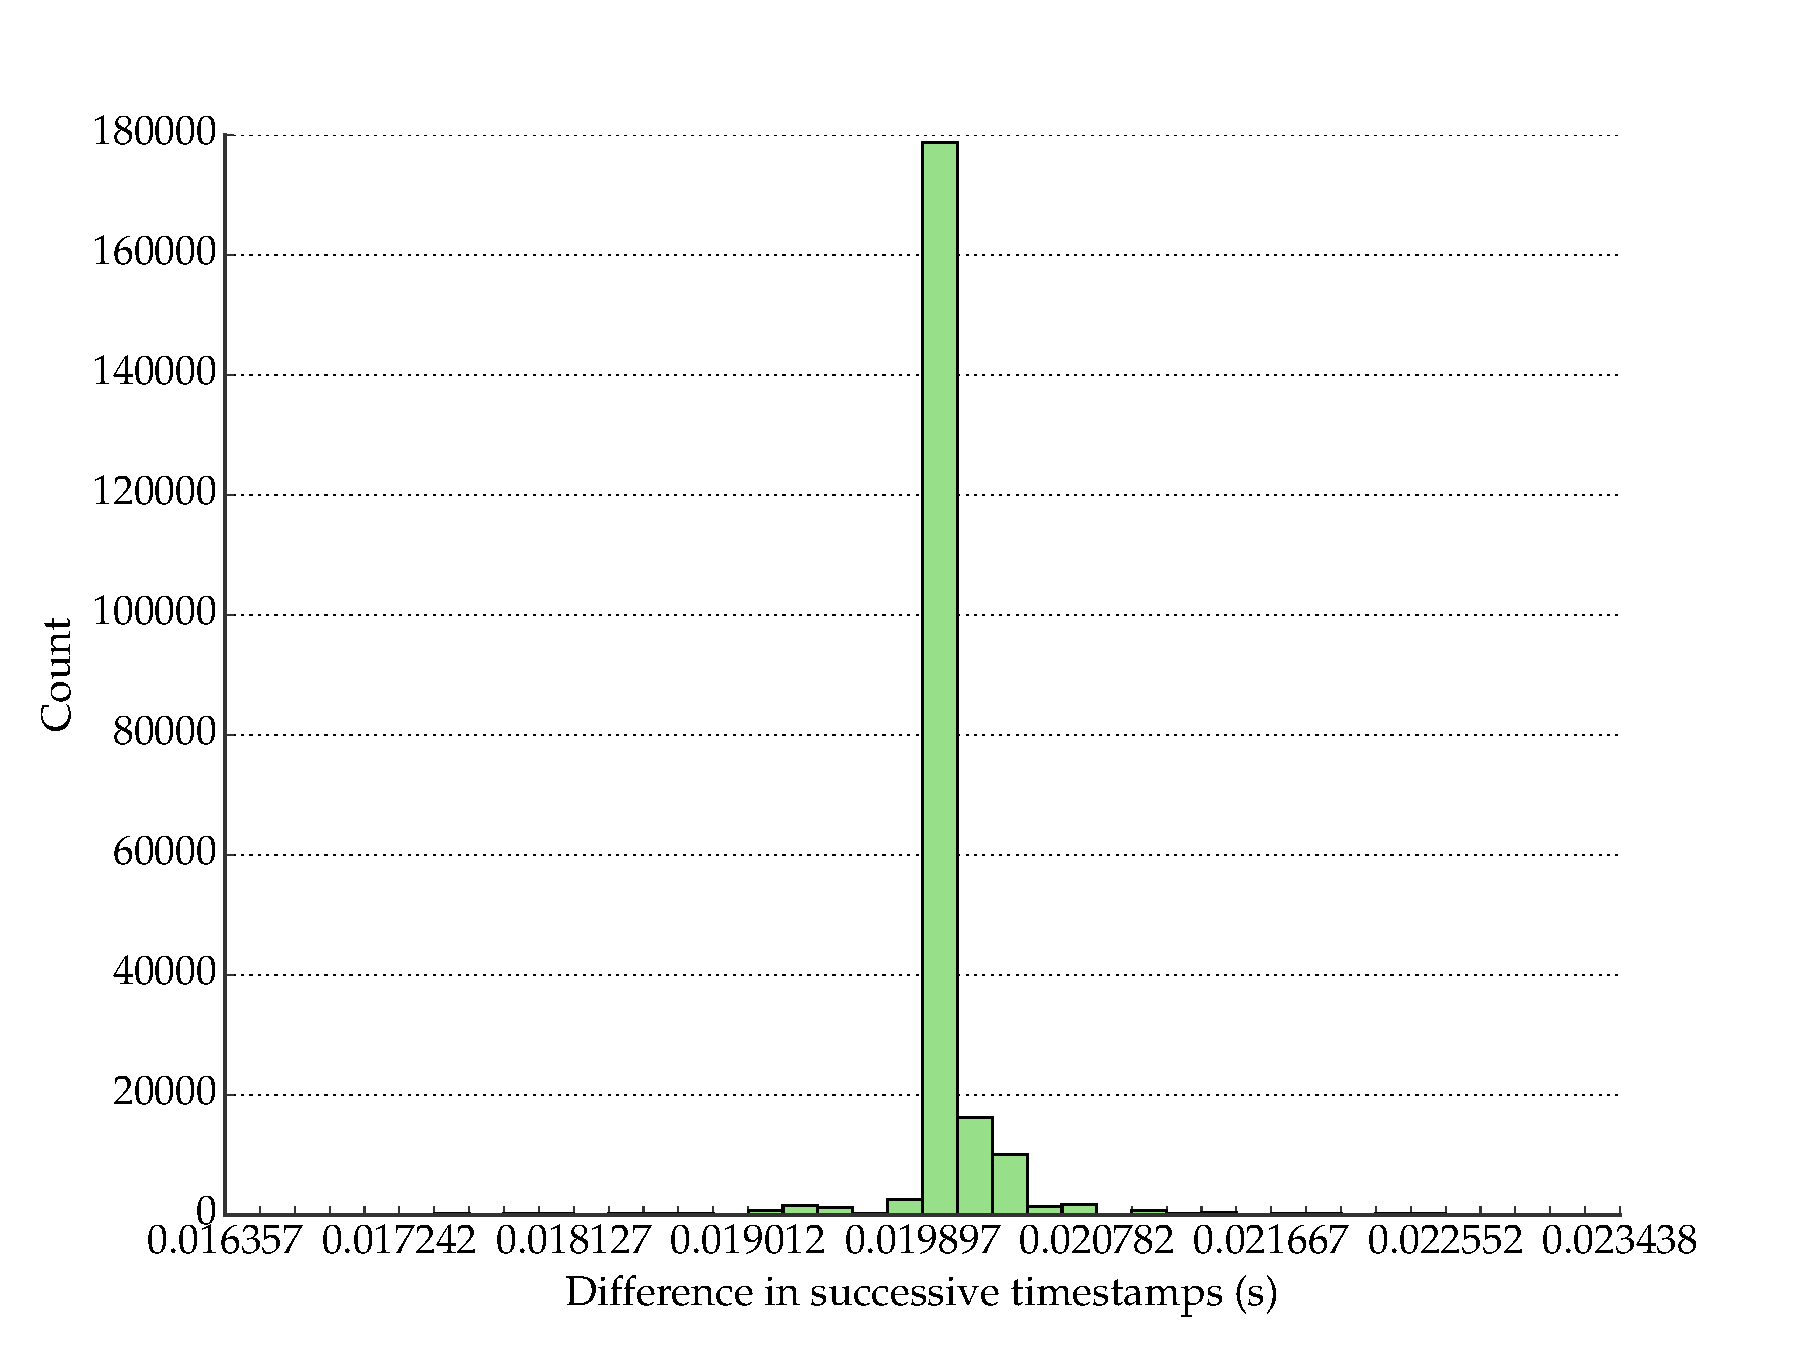
\includegraphics[width=1.0\textwidth]{timestamp_histogram}
        \caption[Histogram of the differences in successive timestamps]{Histogram of the differences in successive timestamps from the data shown in Figure~\ref{fig:x_y_z_flat_plot}. 
            The sample rate was set to 50 \si{Hz}. 0.02002s accounted for 75\% of the 
            differences.
            Thus the actual sample rate is approximately the user-suggested sample rate.}
        \label{fig:timestamp-differences}
      \end{figure}
      
      Android provides both acceleration and linear acceleration sensors, related by 
      $$\textrm{acceleration} = \textrm{linear acceleration} + \textrm{gravity}$$
      They each provide a timestamp represented as a 64-bit integer (i.e. a long) and three 32-bit float values representing the 
      acceleration of each axis in \si{\metre\per\square\second} at that timestamp.   
      Table~\ref{tab:data-row} gives a graphical representation of the data returned.
      
      \begin{table}
        \tabcolsep=0.11cm
        \centering
        \begin{tabu} to \linewidth {|X[2,c] | X[c] | X[c] | X[c] |}
          \hline
          Timestamp & X acceleration & Y acceleration & Z acceleration \\
          \si{ns} & \si{\metre\per\square\second} & \si{\metre\per\square\second} & \si{\metre\per\square\second} \\
          Long & Float & Float & Float \\
          2 bytes & 1 byte & 1 byte & 1 byte \\
          \hline
        \end{tabu}
        \caption{Data from the accelerometer sensor provided to the \texttt{onSensorChanged()} 
            method.}
        \label{tab:data-row}
      \end{table}
      
      Curiously, the timestamp returned as part of the data is documented only as ``The time in nanosecond [sic] at which the event happened'' \cite{androidsensoreventapi}. Further exploration reveals that the timestamp is not defined against any particular zero-base, but rather the time since the device was powered on \cite{androidissuedocumentationbug, androidissuehardwarebug}. The implication of this for the project is that while the timestamp can be relied on for intervals between measurements, it cannot be used between different sets of recordings or across devices.
      
      %TODO: which are the x y z values of the device's accelerometer?

    \subsection{Android Wear Data API}
      \label{sec:prep-data-api}
      As discussed in Section~\ref{sec:smartwatch}, the only radio present in the Samsung Galaxy 
      Gear Live is Bluetooth. To transfer any recorded data from the watch, it must first be transferred to the paired smartphone. 
      The Android Wearable Data Layer API allows communication between Android handheld and wearable
      devices. It provides three methods of communication between devices:
      \begin{description}
        \item[Data items] provide data storage with automatic syncing;
        \item[Messages] are good for remote procedure calls but do not carry data;
        \item[Asset objects] for sending binary blobs of data.
      \end{description}
      
      The project makes use of Assets to send the accelerometer data and Messages to indicate that a particular device has started recording. Use of this API is described in Section~\ref{sec:Transmitting_accelerometer_data}.
      
      %TODO: explain this as a diagram with state machine: recording state, recording off state
      The data layer synchronises data between the handheld and wearable. To do so, the Wearable Data Layer API requires the registration of a listener service, much like the Sensor API. The listener service listens for data layer events, such as the creation of asset objects or when messages are received.      
      
  \section{Choice of tools}
    \subsection{Programming languages}
      \label{sec:programming_languages}
      Java is the native programming language used on Android. Although it is
      possible to write code for Android in programming languages other than Java, for example 
      by using the Android Native Development Kit, doing so would add much complexity for marginal performance gain that is not required. Using a language other than Java would lead to rewrites of many of the Android APIs The Android SDK builds on the principles of Java but is complicated by having to manage interactions with the Android operating system.
      
      XML is Android's standard markup language. All user-interface components are written in XML.
      The project includes a user interface on both the phone and the watch to configure and control the recording of data.
      
      Python 3.4 was chosen as the data processing language due to its ease of use and the strength of its data processing, signal processing and machine learning libraries:
      \begin{description}
        \item[NumPy:] a scientific computing library and the basis for the other three libraries below\cite{van2011numpy}.
        \item[Pandas:] extensions to NumPy that enable easier processing of time-series data\cite{pandas}.
        \item[SciPy:] signal processing tools and other statistical features\cite{scipy}.
        \item[Scikit Learn:] machine learning classifiers and utilities to work with them\cite{scikitlearn}.
      \end{description}
      All of NumPy, SciPy, Pandas and Scikit Learn are open-source and licensed under the BSD license.
    \subsection{Development Environment}
      Two IDEs, Android Studio and PyCharm were used for the development of the Android app and the Python data pipeline respectively. Android Studio is available for free from Google, while PyCharm is provided free for educational use by JetBrains. Both include advanced debuggers.
      
      Though the Android SDK contains a device emulator, it runs slowly and cannot simulate sensors. Developing the Android apps is therefore done by connecting them to a computer and running new versions of the code. This also enables access to the device's logs from the development environment. I made extensive use of logging to determine that the program was executing as expected.
  \section{Software engineering techniques}
    \subsection{Development methodologies}
      I used a combination of development methodologies for the project. The data collection apps were developed using a waterfall methodology, while the data processing was developed using an Agile methodology.
      
      Waterfall models are excellent when the end goals of the project are known and can be well specified. The goal of the data collection apps can be easily stated: to write apps for the smartphone and smartwatch that will allow user collection of accelerometer data.
      
      The data processing and machine learning elements of the project required an Agile methodology. The goal here is less well defined --- to classify activities with the greatest accuracy --- and the implementation to achieve the goal is far more experimental.
      
    \subsection{Version control and backups}
      I used three separate Git repositories for the data collection code\footnote{https://github.com/geotho/WearableActivityClassificationApp}, the data processing code\footnote{https://github.com/geotho/Wearable-Activity-Classifier-Machine-Learning} and the dissertation\footnote{https://github.com/geotho/Wearable-Activity-Classification-Dissertation} respectively. The Git repositories were synced to GitHub at each commit. Version control allowed me to follow a \emph{implement--test--commit} pattern when writing code. 
      
      GitHub also served as one method of backup. Each GitHub repository is publicly accessible such that I can continue implementation even if my primary development computer crashed and I was also locked out of my GitHub account. In addition, I backed up periodically to Dropbox and to an external hard drive. The external hard drive backup retained old copies of files when they were updated. This gives four replications of my entire project, with two of these able to access previous versions of the code.
  \section{Activities for classification}
    \label{sec:activities_for_classification}
    Activities can vary in the amount of movement required, their typical body position and the parts of the body which are moving. When picking activities I wanted to attempt to classify, I wanted to select a mix of activities that were similar in some characteristics and that varied in others.
    
    The activities selected fit into three broad categories:
    \begin{itemize}
      \item physical activities requiring whole body motion;
      \item activities that primarily require arm motion;
      \item low energy upright activities.
    \end{itemize}
    
    The activities that I hope to classify are as follows:
    \begin{itemize}
      \item Physical activities requiring whole body motion:
      \begin{itemize}
        \item Climbing
        \item Cycling
        \item Gym cycling
        \item Running
        \item Stair climbing
        \item Walking
      \end{itemize} 
      \item Activities that primarily require arm motion:
      \begin{itemize}
        \item Computer use
        \item Eating
        \item Playing fussball
      \end{itemize}
      \item Low energy upright activities:
      \begin{itemize}
        \item Gallery perusal
        \item Standing
        \item Teeth brushing
      \end{itemize}
    \end{itemize}
    
  \section{Summary}
    In this section I presented:
    \begin{itemize}
      \item an overview of digital signal processing;
      \item information on the smartphone and smartwatch used;
      \item details of key APIs used including the Android Sensor API and the Android Wear Data API;
      \item development tools and software engineering techniques;
      \item activities I seek to classify.
    \end{itemize}


\chapter{Implementation}
  \section{Data collection}
    This section contains details of the components built to access the accelerometer data and transfer it to a computer.
    
    Because both the smartwatch and the smartphone both run Android, it is possible to create components that are shared between the devices, reducing the amount of code I am required to write and to test, resulting in less redundancy, less complexity and ultimately a more reliable implementation. Both the \texttt{AccelerometerListenerService} and the \texttt{AccelerometerDataBlob} are shared between both devices.
    
    \subsection{Accessing the accelerometer}
      The \texttt{AccelerometerListenerService} is responsible for receiving readings from the accelerometer and delivering them to the data structure responsible for storage.
      
      As described in Section~\ref{sec:sensor-api}, the Sensor API utilises a listener methodology. It is required to create and register a listener that implements \texttt{onSensorChanged()}. 
      
      \subsubsection{Performance considerations}
        Because the accelerometer can update its values at a rate of over 50\si{Hz}, it is vital that any implementation of \texttt{onSensorChanged()} be non-blocking and ideally be very quick to execute. Any expensive computation or IO operation has to be moved to a separate thread.
        
        If the execution of \texttt{onSensorChanged()} takes longer than $\frac{1}{\mathrm{sample-rate}}$, requests for \texttt{onSensorChanged()} will queue and eventually lead to exhaustion of memory or dropping of data.
        
        For this reason the data structure used, discussed in Section~\ref{sec:storing-accelerometer-data}, is very lightweight and \texttt{onSensorChanged()} is only responsible for passing data to it.
      
      \subsubsection{Concurrency considerations}
        Because \texttt{onSensorChanged()} can be called at such a high rate, it is possible that new calls to the method can be made while previous calls are still executing. Data corruption could result from improper handling of asynchronicity.
      
        The documentation for the Sensor API is not explicit about whether calls to \texttt{onSensorChanged()} queue on the same thread or whether they can be dispatched asynchronously. For this reason, the \texttt{AccelerometerListenerService} was designed to be thread-safe by using Java concurrency primatives.
      
      \subsubsection{Power consumption considerations}
        Recording data from the accelerometer can be computationally expensive. This increase in computational overhead translates to an increase in power consumption in battery powered devices such as the smartphone and the smartwatch. It is for this reason that care should be taken to minimise power usage where possible while still collecting all the required data.
        
        One tradeoff that had to be made was between collection strategies. One strategy is to record data at a specified sample rate from when the recording is turned on until it is turned off. An alternative strategy is to record a window of data at set intervals and sleep the remainder of the time. For example, one might set the accelerometer to record 10 seconds of data every 50 seconds.
        
        Though this strategy saves battery power as the device turns off the accelerometer between recordings, a continous recording approach was taken in this project in order to have as much data as possible with which to train. In addition, the battery life was not severly impeded by the continous recording approach.
        
        Typically, Android will power off the display and later the CPU after a period of user-inactivity. Powering off the CPU means that the device will stop recording accelerometer data, and so it is required to maintain a wake-lock which keeps the CPU from powering off. It is also important to remember to release the wake-lock once accelerometer recording is complete. Otherwise, the device's CPU will remain on even when the device appears to be on standby, using battery.
        
      \subsubsection{Sampling rate}
        In ideal conditions, it would be sensible to sample at as fast a rate as possible: the resultant data can always be downsampled afterwards if it is not required. As per the Nyquist-Shannon sampling theory, discussed in Section~\ref{sec:intro-sig-processing}, our sample rate should be greater than twice the highest frequency of the signal. Because it isn't possible to know what the highest frequency is going to be, it would be reasonable to sample at a far higher rate. 
        
        However, picking a very fast sample rate in this context has two potential downsides: battery life drain and the size of resultant data. I investigated whether either battery life or the size of the resulting data would be a limiting factor of sample rate.
        
        The impact on power consumption of increasing the sample rate was negliable. One possible reason for this is that sampling using the accelerometer at all has high fixed costs and increasing the sample rate has lower marginal costs.
      
        Recall from Table~\ref{tab:data-row} that each measurement has a total size of 20 bytes. At a sample rate of 50\si{Hz}, we produce data at approximately 1 KBps or 3.6 MB per hour. The most memory-constrained device is the smartwatch, which only has 512 MB of RAM but 4 GB of internal storage. A data structure that stores the accelerometer data to the internal storage rather than to memory is required, but a sample rate of 50\si{Hz} produces a storable amount of data on reasonable-length activity recording.
        
        Another potential concern regarding data size is the transfer from the smartwatch to the smartphone. The only connection available is Bluetooth. The Bluetooth connection empircally has a maximum transfer rate of no more than 150 KBps, meaning an hour of activity data will take approximately 30 seconds to transfer.

    \subsection{Storing accelerometer data}
      \label{sec:storing-accelerometer-data}
      The data structure to hold the accelerometer data is required to be:
      \begin{itemize}
        \item \textbf{fast} because it will be accessed many times per second and cannot block;
        \item \textbf{on-disk} rather than in-memory, because the smartwatch may not have enough free memory to store all the accelerometer data for lengthy recordings;
        \item \textbf{thread-safe} as it is unclear whether calls to \texttt{onSensorChanged()} are queued or concurrent.
      \end{itemize}
      
      The data structure decided on was a temporary random-access file with buffered writing. The data is written as bytes through an output buffer. The output buffer is maintained in memory and is flushed when it reaches capacity. The capacity of the output buffer was set to 20000 bytes as data is only written in multiples of 20 bytes and the smartwatch is comfortably able to keep 20 kb in memory. This equates to data being saved to disk approximately every 20 seconds.
      
      % data structure – binary data
      % local temporary internal storage as opposed to memory
      % delete when transmitted
    \subsection{Transmitting accelerometer data}
      The accelerometer data has to be transmitted from the smartwatch to the smartphone before it can be transferred to a computer. As discussed in Section~\ref{sec:prep-data-api}, there are two methods to transfer data between the smartwatch and the smartphone: a DataItem and an Asset. Their advantages and disadvantages with respect to this project are highlighted in Table~\ref{tab:dataitem-vs-asset}.
      
      \begin{table}
        \centering
        {\tabulinesep=1.2mm
        \begin{tabu} to \linewidth { X[2,c,m] | X[3,l,m] | X[3,l,m] | }
          & \textbf{DataItem} & \textbf{Asset} \\
          \hline
          \textbf{Advantages} & 
            \begin{itemize}
              \item no separate data fetching step
              \item simpler, more reliable receiver code
              \item negligable transmission time
            \end{itemize} &
            \begin{itemize}
              \item no hard size limit
              \item can create an Asset from a File without storing it in memory
            \end{itemize} \\
          \hline
          \textbf{Disadvantages} &
            \begin{itemize}
              \item 100 KB size limit
              \item have to insert byte arrays
            \end{itemize} &
            \begin{itemize}
              \item some constructors don't seem to work
              \item transmission of large files takes a noticable amount of time
            \end{itemize} \\
          \hline
        \end{tabu}}
        \caption{Advantages and disadvantages of using the \texttt{DataItem} and \texttt{Asset} to transmit data from the smartwatch to the smartphone.}
        \label{tab:dataitem-vs-asset}
      \end{table}
      
      Because the DataItem has a 100 KB limit, an alternate transmission and storage system would have to have been built, where the smartwatch collects 100 KB of data and sends that to the smartphone while it continues to record. It is then reassembled at the smartphone receiver.
      
      I consider this solution inferior to the Asset implementation, which allows transmission of any size of data.
      % DataItem has 100kb limit.
      % Bug with Asset class – FileDescriptor
      % Use of Asset transmit
      % Sender
      % Receiver
    \subsection{User interface}
      \subsubsection{Smartphone}
      
      \subsubsection{Smartwatch}
      
  \section{Activities and data collection method}
    \subsection{Computer use}
    \subsection{Walking}
    \subsection{Cycling}
    \subsection{Standing}
    \subsection{Playing fussball}
    \subsection{Stair climbing}
  \section{Data processing}
    \subsection{Importing and preprocessing}
      \subsubsection{Import}
        %read bytes
        %database
      \subsubsection{Preprocessing}
        %disregard first and last 10 seconds
        %magnitude
        %filtering
      \subsubsection{Binning}
        %10 second overlapping bins
    \subsection{Feature extraction}
    \subsection{Machine learning}
  \section{Summary}


% \chapter{Preparation}
%
% This chapter is empty!
%
% \chapter{Implementation}
%
% empty
%
% \section{Tables}
%
% \begin{samepage}
% Here is a simple example\footnote{A footnote} of a table.
%
% \begin{center}
% \begin{tabular}{l|c|r}
% Left      & Centred & Right \\
% Justified &         & Justified \\[3mm]
% %\hline\\%[-2mm]
% First     & A       & XXX \\
% Second    & AA      & XX  \\
% Last      & AAA     & X   \\
% \end{tabular}
% \end{center}
%
% \noindent
% There is another example table in the proforma.
% \end{samepage}
%
% \chapter{Evaluation}
%
% \section{Printing and binding}
%
% Use a ``duplex'' laser printer that can print on both sides to print
% two copies of your dissertation. Then bind them, for example using the
% comb binder in the Computer Laboratory Library.
%
% \chapter{Conclusion}
%
% I hope that this rough guide to writing a dissertation is \LaTeX\ has
% been helpful and saved you time.


%%%%%%%%%%%%%%%%%%%%%%%%%%%%%%%%%%%%%%%%%%%%%%%%%%%%%%%%%%%%%%%%%%%%%
% the bibliography
\addcontentsline{toc}{chapter}{Bibliography}
\printbibliography

\end{document}
